\documentclass[a4paper]{article}
\addtolength{\hoffset}{-2.25cm}
\addtolength{\textwidth}{4.5cm}
\addtolength{\voffset}{-3.25cm}
\addtolength{\textheight}{5cm}
\setlength{\parskip}{0pt}
\setlength{\parindent}{0in}

%----------------------------------------------------------------------------------------
%	PACKAGES AND OTHER DOCUMENT CONFIGURATIONS
%----------------------------------------------------------------------------------------

\usepackage{blindtext} % Package to generate dummy text
\usepackage{charter} % Use the Charter font
\usepackage[utf8]{inputenc} % Use UTF-8 encoding
\usepackage{microtype} % Slightly tweak font spacing for aesthetics
\usepackage[english, ngerman]{babel} % Language hyphenation and typographical rules
\usepackage{amsthm, amsmath, amssymb} % Mathematical typesetting
\usepackage{float} % Improved interface for floating objects
\usepackage[final, colorlinks = true,
            linkcolor = black,
            citecolor = black]{hyperref} % For hyperlinks in the PDF
\usepackage{graphicx, multicol} % Enhanced support for graphics
\graphicspath{ {./images/} } % Set a graphic path
\usepackage{xcolor} % Driver-independent color extensions
\usepackage{marvosym, wasysym} % More symbols
\usepackage{rotating} % Rotation tools
\usepackage{censor} % Facilities for controlling restricted text
\usepackage{listings, style/lstlisting} % Environment for non-formatted code, !uses style file!
\usepackage{pseudocode} % Environment for specifying algorithms in a natural way
\usepackage{style/avm} % Environment for f-structures, !uses style file!
\usepackage{booktabs} % Enhances quality of tables
\usepackage{tikz-qtree} % Easy tree drawing tool
\tikzset{every tree node/.style={align=center,anchor=north},
         level distance=2cm} % Configuration for q-trees
\usepackage{style/btree} % Configuration for b-trees and b+-trees, !uses style file!
\usepackage[backend=biber,style=numeric,
            sorting=nyt]{biblatex} % Complete reimplementation of bibliographic facilities
\addbibresource{ecl.bib}
\usepackage{csquotes} % Context sensitive quotation facilities
\usepackage[yyyymmdd]{datetime} % Uses YEAR-MONTH-DAY format for dates
\renewcommand{\dateseparator}{-} % Sets dateseparator to '-'
\usepackage{fancyhdr} % Headers and footers
\pagestyle{fancy} % All pages have headers and footers
\fancyhead{}\renewcommand{\headrulewidth}{0pt} % Blank out the default header
\fancyfoot[L]{} % Custom footer text
\fancyfoot[C]{} % Custom footer text
\fancyfoot[R]{\thepage} % Custom footer text
\newcommand{\note}[1]{\marginpar{\scriptsize \textcolor{red}{#1}}} % Enables comments in red on margin

%----------------------------------------------------------------------------------------

\begin{document}


%-------------------------------
%	TITLE SECTION
%-------------------------------

\fancyhead[C]{}
\hrule \medskip % Upper rule
\begin{minipage}{0.295\textwidth}
\raggedright
\footnotesize
Sotirios Moschos \hfill\\
9030\hfill\\
moschoss@ece.auth.gr
\end{minipage}
\begin{minipage}{0.4\textwidth}
\centering
\large
Homework Assignment 1\\
\normalsize
Advanced Signal Processing, 20/21\\
\end{minipage}
\begin{minipage}{0.295\textwidth}
\raggedleft
\today\hfill\\
\end{minipage}
\medskip\hrule
\bigskip

%-------------------------------
%	CONTENTS
%-------------------------------

\section{First Exercise}
The first exercise given is the following:

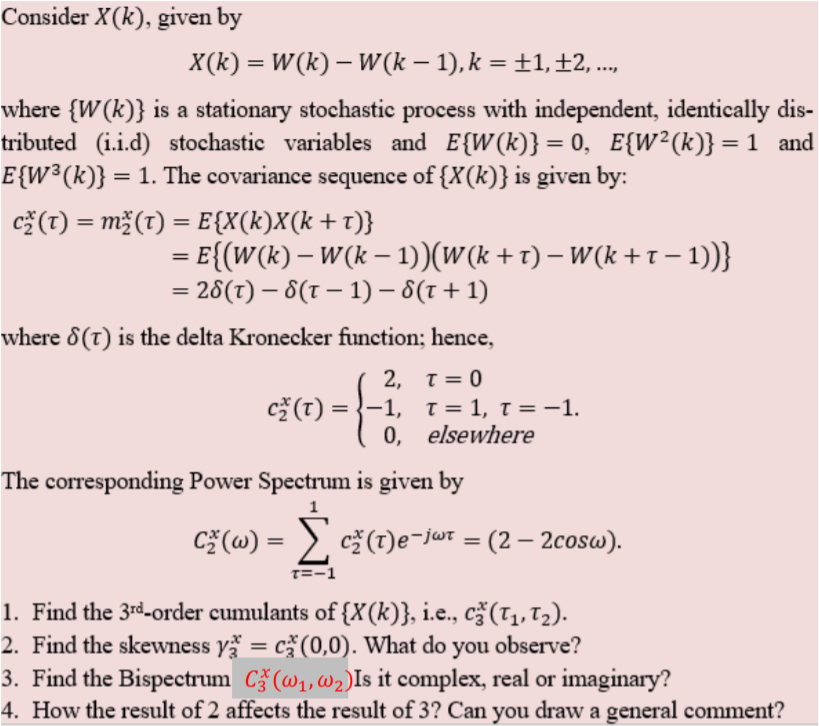
\includegraphics{Images/ASP_HW1.PNG}

\subsection{First Sub-task}

At first, we compute the 3rd order cumulants of X(k).
\begin{equation*}
\begin{aligned}
c_3^x(\tau1,\tau2) &= m_3^x(\tau1,\tau2)-m_1^x[m_2^x(\tau1)+m_2^x(\tau2)+m_2^x(\tau2-\tau1)]+2(m_1^x)^3 \\
&= m_3^x(\tau1,\tau2) \text{ because } m_1^x=E[X(k)]=E[W(k)]-E[W(k-1)]=0 \\
\end{aligned}
\end{equation*}

Hence,
\begin{equation*}
\begin{aligned}
c_3^x(\tau1,\tau2) &= m_3^x(\tau1,\tau2) = E(X(k)X(k+\tau1)X(k+\tau2)) \\
&= E((W(k)-W(k-1)(W(k+\tau1))-W(k+\tau1-1))(W(k+\tau2)-W(k+\tau2-1))) \\
&= E(W(k)W(k+\tau1)W(k+\tau2)-W(k)W(k+\tau1)W(k+\tau2-1)-W(k)W(k+\tau1-1)W(k+\tau2) \\
&+ W(k)W(k+\tau1-1)W(k+\tau2-1)-W(k-1)W(k+\tau1)W(k+\tau2)+W(k-1)W(k+\tau1-1)W(k+\tau2) \\
&+ W(k-1)W(k+\tau1)W(k+\tau2-1)-W(k-1)W(k+\tau1-1)W(k+\tau2-1)) \\
&= E(W(k)W(k+\tau1)W(k+\tau2))-E(W(k)W(k+\tau1)W(k+\tau2-1))-E(W(k)W(k+\tau1-1)W(k+\tau2)) \\
&+ E(W(k)W(k+\tau1-1)W(k+\tau2-1))-E(W(k-1)W(k+\tau1)W(k+\tau2)) \\
&+ E(W(k-1)W(k+\tau1-1)W(k+\tau2))+E(W(k-1)W(k+\tau1)W(k+\tau2-1)) \\
&- E(W(k-1)W(k+\tau1-1)W(k+\tau2-1)) \\ \\
& W(k),W(k+\tau) \text{ are independent stochastic processes.Thus, } E(W(k)W(k+\tau))=E(W(k)E(W(k+\tau)) \\
\end{aligned}
\end{equation*}

Hence,
\begin{equation*}
\begin{aligned}
c_3^x(\tau1,\tau2) &= -\delta(\tau1,\tau2-1)-\delta(\tau1-1,\tau2) \\
&+ \delta(\tau1-1,\tau2-1)-\delta(\tau1+1,\tau2+1) \\
&+ \delta(\tau1+1,\tau2-1)+\delta(\tau1,\tau2+1) \\
&= \begin{cases}
    -1, & \tau1=0,\tau2=1 \\
    -1, & \tau1=1,\tau2=0 \\
    +1, & \tau1=1,\tau2=1 \\
    -1, & \tau1=-1,\tau2=-1 \\
    +1, & \tau1=-1,\tau2=0 \\
    +1 & \tau1=0,\tau2=-1 \\
    \end{cases}
\end{aligned}
\end{equation*}

\subsection{Second Sub-task}
To find the skewness we observe the 3rd order cumulants in \((\tau1,\tau2)=(0,0)\).\\Hence,
\[\gamma_3^x=c_3^x(0,0)=0\]
We can state that the stochastic process X(k) has a probability distribution where the observations are perfectly symmetrical around the mean.So, \((m_1^x=0)\) and the observations are symmetrical around (0,0).

\subsection{Third Sub-task}
\begin{equation*}
\begin{aligned}
C_3^x(\omega1,\omega2) &= \sum_{\tau1=-1}^{\tau1=+1}\sum_{\tau2=-1}^{\tau2=+1}c_3^x(\tau1,\tau2)
e^{-j(\omega1\tau1+\omega2\tau2)} \text{ where, } |\omega1|\leq\pi, |\omega2|\leq\pi,
|\omega1+\omega2|\leq\pi \\
&= e^{-j(\omega1+\omega2)}-e^{-j(-\omega1-\omega2)}\\
&+ e^{j\omega1} + e^{-j\omega2} - e^{-j\omega1} - e^{-j\omega2}\\
&= -2j(-\sin{\omega1}) - 2j(-\sin{\omega2}) - 2j(\sin{(\omega1+\omega2)})\\
&= 2j(\sin{\omega1}+\sin{\omega2}-\sin{(\omega1+\omega2)})
\end{aligned}
\end{equation*} \\
Hence, the bispectrum \(C_3^x(\omega1,\omega2)\) is imaginary.

\subsection{Fourth Sub-task}
If \(c_3^x(\tau1,\tau2)\neq0\) there will be a real part in the bispectrum apart from the imaginary.
So, we can assume that the skewness of X(k) determines the real part of the bispectrum.


\end{document}
